\section{ចម្លើយប៉ារ៉ាបូល}
%
\begin{enumerate}
  \item គូសប៉ារ៉ាបូលដោយមានកំណុំ និងបន្ទាត់ប្រាប់ទិស៖
  \begin{Enumerate}(2)
    \item $ F(1,0) $ និង $ (\Delta):x=-1 $\\
      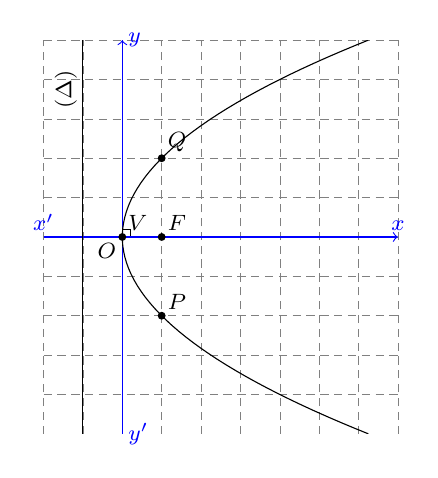
\begin{tikzpicture}[%
      scale=.5,%
      every node/.append style={font=\footnotesize,inner sep=2pt}]
      \coordinate(O)at(0,0);
      \coordinate(x')at(-2,0);\coordinate(x)at(7,0);
      \coordinate(y')at(0,-5);\coordinate(y)at(0,5);
      \coordinate(B)at(-2,-5);\coordinate(E)at(7,5);
      \coordinate(d')at(-1,-5);\coordinate(d)at(-1,5);
      \coordinate(F)at(1,0);\coordinate(V)at(0,0);
      \coordinate(P)at(1,-2);\coordinate(Q)at(1,2);
      \draw(.2,0)--(.2,.2)--(0,.2);
      \node[below left]at(O){$ O $};
      \draw[help lines,densely dashed](B) grid (E);
      \draw[->,color=blue](x')node[above]{$ x' $}--(x)node[above]{$ x $};
      \draw[->,color=blue](y')node[right]{$ y' $}--(y)node[right]{$ y $};
      \draw(d')--node[sloped,very near end,above]{$ (\Delta) $}(d);
      \clip(B) rectangle (E);
      \draw[variable=\y,domain=-5:5,samples=70] plot({.25*\y*\y},{\y});
      \foreach\p in {F,V,P,Q}{%
        \fill[color=black](\p)circle(.1)node[above right]{$ \p $};}
      \end{tikzpicture}
    %
    \item $ F(-1,0) $ និង $ (\Delta):x=1 $\\
    %
      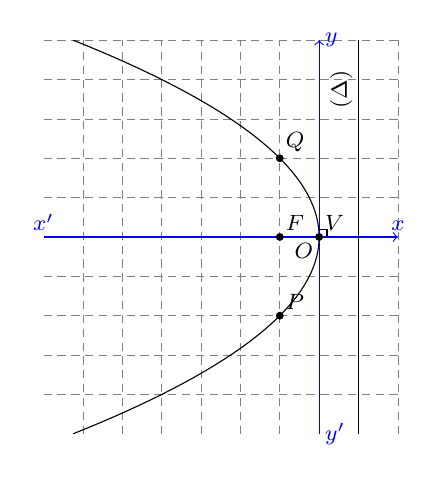
\begin{tikzpicture}[%
      scale=.5,%
      every node/.append style={font=\footnotesize,inner sep=2pt}]
      \coordinate(O)at(0,0);
      \coordinate(x')at(-7,0);\coordinate(x)at(2,0);
      \coordinate(y')at(0,-5);\coordinate(y)at(0,5);
      \coordinate(B)at(-7,-5);\coordinate(E)at(2,5);
      \coordinate(d')at(1,-5);\coordinate(d)at(1,5);
      \coordinate(F)at(-1,0);\coordinate(V)at(0,0);
      \coordinate(P)at(-1,-2);\coordinate(Q)at(-1,2);
      \draw(.2,0)--(.2,.2)--(0,.2);
      \node[below left]at(O){$ O $};
      \draw[help lines,densely dashed](B) grid (E);
      \draw[->,color=blue](x')node[above]{$ x' $}--(x)node[above]{$ x $};
      \draw[->,color=blue](y')node[right]{$ y' $}--(y)node[right]{$ y $};
      \draw(d')--node[sloped,very near end,above]{$ (\Delta) $}(d);
      \clip(B) rectangle (E);
      \draw[variable=\y,domain=-5:5,samples=70] plot({-.25*\y*\y},{\y});
      \foreach\p in {F,V,P,Q}{%
        \fill[color=black](\p)circle(.1)node[above right]{$ \p $};}
      \end{tikzpicture}
    %
    \item $ F(2,1) $ និង $ (\Delta):x=0 $\\
    %
    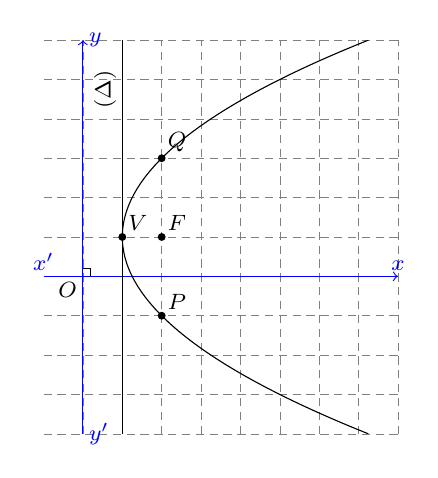
\begin{tikzpicture}[%
    scale=.5,%
    every node/.append style={font=\footnotesize,inner sep=2pt}]
    \coordinate(O)at(0,0);
    \coordinate(x')at(-1,0);\coordinate(x)at(8,0);
    \coordinate(y')at(0,-4);\coordinate(y)at(0,6);
    \coordinate(B)at(-1,-4);\coordinate(E)at(8,6);
    \coordinate(d')at(1,-4);\coordinate(d)at(1,6);
    \coordinate(F)at(2,1);\coordinate(V)at(1,1);
    \coordinate(P)at(2,-1);\coordinate(Q)at(2,3);
    \draw(.2,0)--(.2,.2)--(0,.2);
    \node[below left]at(O){$ O $};
    \draw[help lines,densely dashed](B) grid (E);
    \draw[->,color=blue](x')node[above]{$ x' $}--(x)node[above]{$ x $};
    \draw[->,color=blue](y')node[right]{$ y' $}--(y)node[right]{$ y $};
    \draw(d')--node[sloped,very near end,above]{$ (\Delta) $}(d);
    \clip(B) rectangle (E);
    \draw[variable=\y,domain=-4:6,samples=70] plot({.25*(\y*(\y-2)+5)},{\y});
    \foreach\p in {F,V,P,Q}{%
      \fill[color=black](\p)circle(.1)node[above right]{$ \p $};}
    \end{tikzpicture}
    %
    \item $ F(4,2) $ និង $ (\Delta):x=2 $\\
    %
    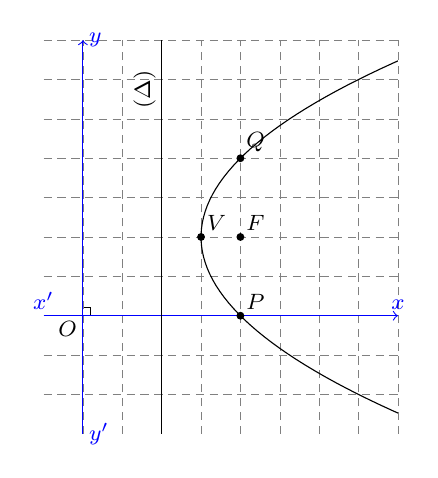
\begin{tikzpicture}[%
    scale=.5,%
    every node/.append style={font=\footnotesize,inner sep=2pt}]
    \coordinate(O)at(0,0);
    \coordinate(x')at(-1,0);\coordinate(x)at(8,0);
    \coordinate(y')at(0,-3);\coordinate(y)at(0,7);
    \coordinate(B)at(-1,-3);\coordinate(E)at(8,7);
    \coordinate(d')at(2,-3);\coordinate(d)at(2,7);
    \coordinate(F)at(4,2);\coordinate(V)at(3,2);
    \coordinate(P)at(4,0);\coordinate(Q)at(4,4);
    \draw(.2,0)--(.2,.2)--(0,.2);
    \node[below left]at(O){$ O $};
    \draw[help lines,densely dashed](B) grid (E);
    \draw[->,color=blue](x')node[above]{$ x' $}--(x)node[above]{$ x $};
    \draw[->,color=blue](y')node[right]{$ y' $}--(y)node[right]{$ y $};
    \draw(d')--node[sloped,very near end,above]{$ (\Delta) $}(d);
    \clip(B) rectangle (E);
    \draw[variable=\y,domain=-3:7,samples=70] plot({.25*(\y*(\y-4)+16)},{\y});
    \foreach\p in {F,V,P,Q}{%
      \fill[color=black](\p)circle(.1)node[above right]{$ \p $};}
    \end{tikzpicture}
    %
    \item $ F(-3,1) $ និង $ (\Delta):x=-2 $\\
    %
    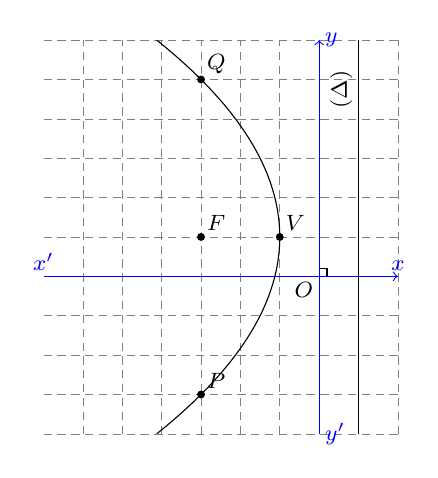
\begin{tikzpicture}[%
    scale=.5,%
    every node/.append style={font=\footnotesize,inner sep=2pt}]
    \coordinate(O)at(0,0);
    \coordinate(x')at(-7,0);\coordinate(x)at(2,0);
    \coordinate(y')at(0,-4);\coordinate(y)at(0,6);
    \coordinate(B)at(-7,-4);\coordinate(E)at(2,6);
    \coordinate(d')at(1,-4);\coordinate(d)at(1,6);
    \coordinate(F)at(-3,1);\coordinate(V)at(-1,1);
    \coordinate(P)at(-3,-3);\coordinate(Q)at(-3,5);
    \draw(.2,0)--(.2,.2)--(0,.2);
    \node[below left]at(O){$ O $};
    \draw[help lines,densely dashed](B) grid (E);
    \draw[->,color=blue](x')node[above]{$ x' $}--(x)node[above]{$ x $};
    \draw[->,color=blue](y')node[right]{$ y' $}--(y)node[right]{$ y $};
    \draw(d')--node[sloped,very near end,above]{$ (\Delta) $}(d);
    \clip(B) rectangle (E);
    \draw[variable=\y,domain=-4:6,samples=70] plot({-.125*(\y*(\y-2)+9)},{\y});
    \foreach\p in {F,V,P,Q}{%
      \fill[color=black](\p)circle(.1)node[above right]{$ \p $};}
    \end{tikzpicture}
    %
    \item $ F(0,2) $ និង $ (\Delta):x=1 $\\
    %
    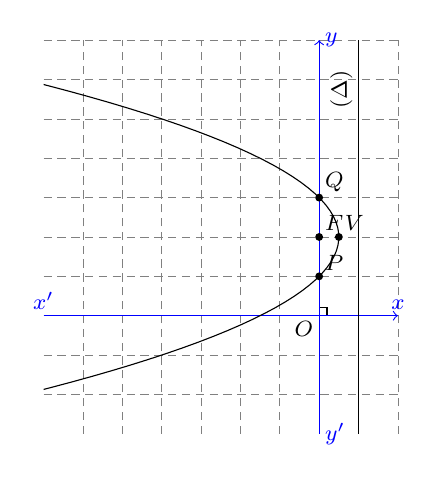
\begin{tikzpicture}[%
    scale=.5,%
    every node/.append style={font=\footnotesize,inner sep=2pt}]
    \coordinate(O)at(0,0);
    \coordinate(x')at(-7,0);\coordinate(x)at(2,0);
    \coordinate(y')at(0,-3);\coordinate(y)at(0,7);
    \coordinate(B)at(-7,-3);\coordinate(E)at(2,7);
    \coordinate(d')at(1,-3);\coordinate(d)at(1,7);
    \coordinate(F)at(0,2);\coordinate(V)at(.5,2);
    \coordinate(P)at(0,1);\coordinate(Q)at(0,3);
    \draw(.2,0)--(.2,.2)--(0,.2);
    \node[below left]at(O){$ O $};
    \draw[help lines,densely dashed](B) grid (E);
    \draw[->,color=blue](x')node[above]{$ x' $}--(x)node[above]{$ x $};
    \draw[->,color=blue](y')node[right]{$ y' $}--(y)node[right]{$ y $};
    \draw(d')--node[sloped,very near end,above]{$ (\Delta) $}(d);
    \clip(B) rectangle (E);
    \draw[variable=\y,domain=-4:6,samples=70] plot({-.5*(\y*(\y-4)+3)},{\y});
    \foreach\p in {F,V,P,Q}{%
      \fill[color=black](\p)circle(.1)node[above right]{$ \p $};}
    \end{tikzpicture}
    %
  \end{Enumerate}
  %
  \item ចូរគូសប៉ារ៉ាបូលដែលមានកំណុំ និងបន្ទាត់ប្រាប់ទិសដូចខាងក្រោម៖
  \begin{Enumerate}(2)
    \item $ F(0,1) $ និង $ (\Delta):y=-1 $\\
    %
    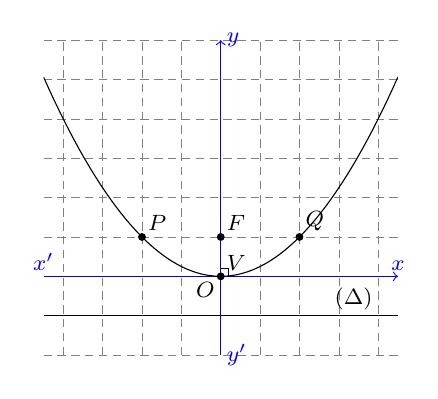
\begin{tikzpicture}[%
    scale=.5,%
    every node/.append style={font=\footnotesize,inner sep=2pt}]
    \coordinate(O)at(0,0);
    \coordinate(x')at(-4.5,0);\coordinate(x)at(4.5,0);
    \coordinate(y')at(0,-2);\coordinate(y)at(0,6);
    \coordinate(B)at(-4.5,-2);\coordinate(E)at(4.5,6);
    \coordinate(d')at(-4.5,-1);\coordinate(d)at(4.5,-1);
    \coordinate(F)at(0,1);\coordinate(V)at(0,0);
    \coordinate(P)at(-2,1);\coordinate(Q)at(2,1);
    \draw(.2,0)--(.2,.2)--(0,.2);
    \node[below left]at(O){$ O $};
    \draw[help lines,densely dashed](B) grid (E);
    \draw[->,color=blue](x')node[above]{$ x' $}--(x)node[above]{$ x $};
    \draw[->,color=blue](y')node[right]{$ y' $}--(y)node[right]{$ y $};
    \draw(d')--node[sloped,very near end,above]{$ (\Delta) $}(d);
    \clip(B) rectangle (E);
    \draw[domain=-4.5:4.5,samples=70] plot({\x},{.25*\x*\x});
    \foreach\p in {F,V,P,Q}{%
      \fill[color=black](\p)circle(.1)node[above right]{$ \p $};}
    \end{tikzpicture}
    %
    \item $ F(0,-1) $ និង $ (\Delta):y=1 $\\
    %
    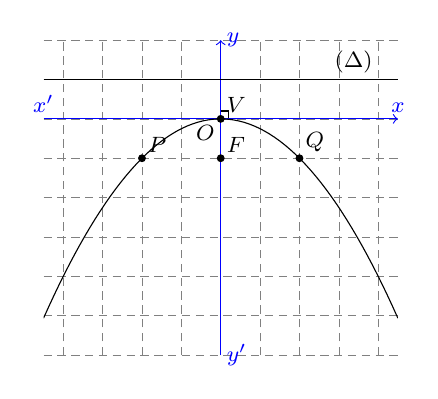
\begin{tikzpicture}[%
    scale=.5,%
    every node/.append style={font=\footnotesize,inner sep=2pt}]
    \coordinate(O)at(0,0);
    \coordinate(x')at(-4.5,0);\coordinate(x)at(4.5,0);
    \coordinate(y')at(0,-6);\coordinate(y)at(0,2);
    \coordinate(B)at(-4.5,-6);\coordinate(E)at(4.5,2);
    \coordinate(d')at(-4.5,1);\coordinate(d)at(4.5,1);
    \coordinate(F)at(0,-1);\coordinate(V)at(0,0);
    \coordinate(P)at(-2,-1);\coordinate(Q)at(2,-1);
    \draw(.2,0)--(.2,.2)--(0,.2);
    \node[below left]at(O){$ O $};
    \draw[help lines,densely dashed](B) grid (E);
    \draw[->,color=blue](x')node[above]{$ x' $}--(x)node[above]{$ x $};
    \draw[->,color=blue](y')node[right]{$ y' $}--(y)node[right]{$ y $};
    \draw(d')--node[sloped,very near end,above]{$ (\Delta) $}(d);
    \clip(B) rectangle (E);
    \draw[domain=-4.5:4.5,samples=70] plot({\x},{-.25*\x*\x});
    \foreach\p in {F,V,P,Q}{%
      \fill[color=black](\p)circle(.1)node[above right]{$ \p $};}
    \end{tikzpicture}
    %
    \item $ F(2,2) $ និង $ (\Delta):y=0 $\\
    %
    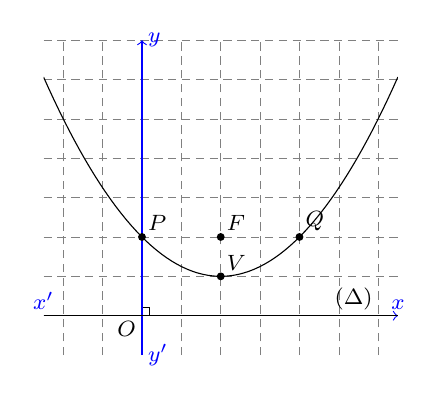
\begin{tikzpicture}[%
    scale=.5,%
    every node/.append style={font=\footnotesize,inner sep=2pt}]
    \coordinate(O)at(0,0);
    \coordinate(x')at(-2.5,0);\coordinate(x)at(6.5,0);
    \coordinate(y')at(0,-1);\coordinate(y)at(0,7);
    \coordinate(B)at(-2.5,-1);\coordinate(E)at(6.5,7);
    \coordinate(d')at(-2.5,0);\coordinate(d)at(6.5,0);
    \coordinate(F)at(2,2);\coordinate(V)at(2,1);
    \coordinate(P)at(0,2);\coordinate(Q)at(4,2);
    \draw(.2,0)--(.2,.2)--(0,.2);
    \node[below left]at(O){$ O $};
    \draw[help lines,densely dashed](B) grid (E);
    \draw[->,color=blue](x')node[above]{$ x' $}--(x)node[above]{$ x $};
    \draw[->,color=blue](y')node[right]{$ y' $}--(y)node[right]{$ y $};
    \draw(d')--node[sloped,very near end,above]{$ (\Delta) $}(d);
    \clip(B) rectangle (E);
    \draw[domain=-2.5:6.5,samples=70] plot({\x},{.25*(\x*(\x-4)+8)});
    \foreach\p in {F,V,P,Q}{%
      \fill[color=black](\p)circle(.1)node[above right]{$ \p $};}
    \end{tikzpicture}
    %
    \item $ F(-1,0) $ និង $ (\Delta):y=2 $\\
    %
    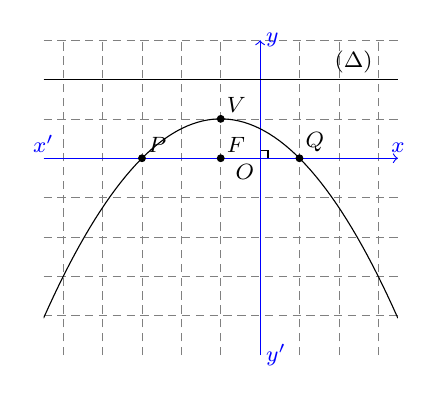
\begin{tikzpicture}[%
    scale=.5,%
    every node/.append style={font=\footnotesize,inner sep=2pt}]
    \coordinate(O)at(0,0);
    \coordinate(x')at(-5.5,0);\coordinate(x)at(3.5,0);
    \coordinate(y')at(0,-5);\coordinate(y)at(0,3);
    \coordinate(B)at(-5.5,-5);\coordinate(E)at(3.5,3);
    \coordinate(d')at(-5.5,2);\coordinate(d)at(3.5,2);
    \coordinate(F)at(-1,0);\coordinate(V)at(-1,1);
    \coordinate(P)at(-3,0);\coordinate(Q)at(1,0);
    \draw(.2,0)--(.2,.2)--(0,.2);
    \node[below left]at(O){$ O $};
    \draw[help lines,densely dashed](B) grid (E);
    \draw[->,color=blue](x')node[above]{$ x' $}--(x)node[above]{$ x $};
    \draw[->,color=blue](y')node[right]{$ y' $}--(y)node[right]{$ y $};
    \draw(d')--node[sloped,very near end,above]{$ (\Delta) $}(d);
    \clip(B) rectangle (E);
    \draw[domain=-5.5:3.5,samples=70] plot({\x},{-.25*(\x*(\x+2)-3)});
    \foreach\p in {F,V,P,Q}{%
      \fill[color=black](\p)circle(.1)node[above right]{$ \p $};}
    \end{tikzpicture}
    %
    \item $ F(1,2) $ និង $ (\Delta):y=-2 $\\
    %
    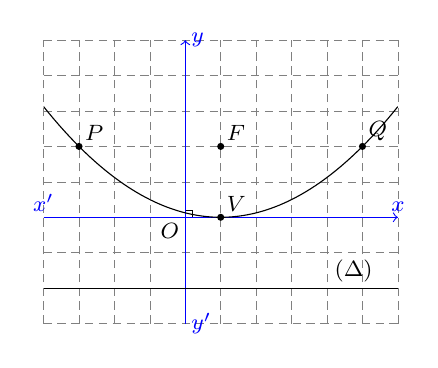
\begin{tikzpicture}[%
    scale=.45,%
    every node/.append style={font=\footnotesize,inner sep=2pt}]
    \coordinate(O)at(0,0);
    \coordinate(x')at(-4,0);\coordinate(x)at(6,0);
    \coordinate(y')at(0,-3);\coordinate(y)at(0,5);
    \coordinate(B)at(-4,-3);\coordinate(E)at(6,5);
    \coordinate(d')at(-4,-2);\coordinate(d)at(6,-2);
    \coordinate(F)at(1,2);\coordinate(V)at(1,0);
    \coordinate(P)at(-3,2);\coordinate(Q)at(5,2);
    \draw(.2,0)--(.2,.2)--(0,.2);
    \node[below left]at(O){$ O $};
    \draw[help lines,densely dashed](B) grid (E);
    \draw[->,color=blue](x')node[above]{$ x' $}--(x)node[above]{$ x $};
    \draw[->,color=blue](y')node[right]{$ y' $}--(y)node[right]{$ y $};
    \draw(d')--node[sloped,very near end,above]{$ (\Delta) $}(d);
    \clip(B) rectangle (E);
    \draw[domain=-4:6,samples=70] plot({\x},{.125*(\x*(\x-2)+1)});
    \foreach\p in {F,V,P,Q}{%
      \fill[color=black](\p)circle(.1)node[above right]{$ \p $};}
    \end{tikzpicture}
    %
    \item $ F(0,1) $ និង $ (\Delta):y=2 $\\
    %
    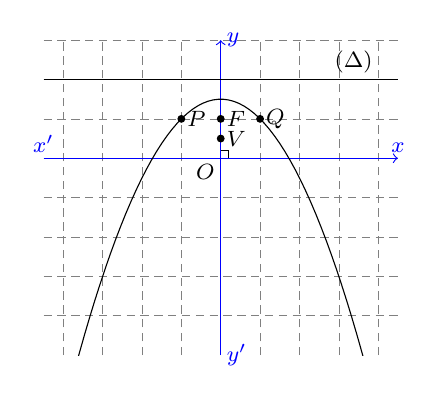
\begin{tikzpicture}[%
    scale=.5,%
    every node/.append style={font=\footnotesize,inner sep=2pt,inner sep=2pt}]
    \coordinate(O)at(0,0);
    \coordinate(x')at(-4.5,0);\coordinate(x)at(4.5,0);
    \coordinate(y')at(0,-5);\coordinate(y)at(0,3);
    \coordinate(B)at(-4.5,-5);\coordinate(E)at(4.5,3);
    \coordinate(d')at(-4.5,2);\coordinate(d)at(4.5,2);
    \coordinate(F)at(0,1);\coordinate(V)at(0,.5);
    \coordinate(P)at(-1,1);\coordinate(Q)at(1,1);
    \draw(.2,0)--(.2,.2)--(0,.2);
    \node[below left]at(O){$ O $};
    \draw[help lines,densely dashed](B) grid (E);
    \draw[->,color=blue](x')node[above]{$ x' $}--(x)node[above]{$ x $};
    \draw[->,color=blue](y')node[right]{$ y' $}--(y)node[right]{$ y $};
    \draw(d')--node[sloped,very near end,above]{$ (\Delta) $}(d);
    \clip(B) rectangle (E);
    \draw[domain=-4.5:4.5,samples=70] plot({\x},{-.5*(\x*\x-3))});
    \foreach\p in {F,V,P,Q}{%
      \fill[color=black](\p)circle(.1)node[right]{$ \p $};}
    \end{tikzpicture}
    %
  \end{Enumerate}
  %
\end{enumerate}